\documentclass[12pt,twoside]{article}
\usepackage[dvipsnames]{xcolor}
\usepackage{tikz,graphicx,amsmath,amsfonts,amscd,amssymb,bm,cite,epsfig,epsf,url}
\usepackage[hang,flushmargin]{footmisc}
\usepackage[colorlinks=true,urlcolor=blue,citecolor=blue]{hyperref}
\usepackage{amsthm,multirow,wasysym,appendix}
\usepackage{array,subcaption} 
% \usepackage[small,bf]{caption}
\usepackage{bbm}
\usepackage{pgfplots}
\usetikzlibrary{spy}
\usepgfplotslibrary{external}
\usepgfplotslibrary{fillbetween}
\usetikzlibrary{arrows,automata}
\usepackage{thmtools}
\usepackage{blkarray} 
\usepackage{textcomp}
\usepackage[left=0.8in,right=1.0in,top=1.0in,bottom=1.0in]{geometry}

\usepackage{times}
\usepackage{amsfonts}
\usepackage{amsmath}
\usepackage{latexsym}
\usepackage{color}
\usepackage{graphics}
\usepackage{enumerate}
\usepackage{amstext}
\usepackage{blkarray}
\usepackage{url}
\usepackage{epsfig}
\usepackage{bm}
\usepackage{hyperref}
\hypersetup{
    colorlinks=true,
    linkcolor=blue,
    filecolor=magenta,      
    urlcolor=blue,
}
\usepackage{textcomp}
\usepackage[left=0.8in,right=1.0in,top=1.0in,bottom=1.0in]{geometry}
\usepackage{mathtools}
\usepackage{minted}


%% Probability operators and functions
%
% \def \P{\mathrm{P}}
\def \P{\mathrm{P}}
\def \E{\mathrm{E}}
\def \Var{\mathrm{Var}}
\let\var\Var
\def \Cov {\mathrm{Cov}} \let\cov\Cov
\def \MSE {\mathrm{MSE}} \let\mse\MSE
\def \sgn {\mathrm{sgn}}
\def \R {\mathbb{R}}
\def \C {\mathbb{C}}
\def \N {\mathbb{N}}
\def \Z {\mathbb{Z}}
\def \cV {\mathcal{V}}
\def \cS {\mathcal{S}}
\DeclareMathOperator*{\argmin}{arg\,min}
\DeclareMathOperator*{\argmax}{arg\,max}
\newcommand{\red}[1]{\textcolor{red}{#1}}
\newcommand{\blue}[1]{\textcolor{blue}{#1}}
\newcommand{\green}[1]{\textcolor{ForestGreen}{ #1}}
\newcommand{\fuchsia}[1]{\textcolor{RoyalPurple}{ #1}}

%
%% Probability distributions
%
%\def \Bern    {\mathrm{Bern}}
%\def \Binom   {\mathrm{Binom}}
%\def \Exp     {\mathrm{Exp}}
%\def \Geom    {\mathrm{Geom}}
%\def \Norm    {\mathcal{N}}
%\def \Poisson {\mathrm{Poisson}}
%\def \Unif    {\mathrm {U}}
%
\newcommand{\bdb}[1]{\textcolor{red}{#1}}

\newcommand{\ml}[1]{\mathcal{ #1 } }
\newcommand{\wh}[1]{\widehat{ #1 } }
\newcommand{\wt}[1]{\widetilde{ #1 } }
\newcommand{\conj}[1]{\overline{ #1 } }
\newcommand{\rnd}[1]{\tilde{ #1 } }
\newcommand{\rv}[1]{ \rnd{ #1}  }
\newcommand{\rx}{\rnd{ x}  }
\newcommand{\ry}{\rnd{ y}  }
\newcommand{\ra}{\rnd{ a}  }
\newcommand{\rb}{\rnd{ b}  }
\newcommand{\rpc}{\widetilde{ pc}  }

\def \cnd {\, | \,}
\def \Id { I }
\def \J {\mathbf{1}\mathbf{1}^T}

\newcommand{\op}[1]{\operatorname{#1}}
\newcommand{\setdef}[2]{ := \keys{ #1 \; | \; #2 } }
\newcommand{\set}[2]{ \keys{ #1 \; | \; #2 } }
\newcommand{\sign}[1]{\op{sign}\left( #1 \right) }
\newcommand{\trace}[1]{\op{tr}\left( #1 \right) }
\newcommand{\tr}[1]{\op{tr}\left( #1 \right) }
\newcommand{\inv}[1]{\left( #1 \right)^{-1} }
\newcommand{\abs}[1]{\left| #1 \right|}
\newcommand{\sabs}[1]{| #1 |}
\newcommand{\keys}[1]{\left\{ #1 \right\}}
\newcommand{\sqbr}[1]{\left[ #1 \right]}
\newcommand{\sbrac}[1]{ ( #1 ) }
\newcommand{\brac}[1]{\left( #1 \right) }
\newcommand{\bbrac}[1]{\big( #1 \big) }
\newcommand{\Bbrac}[1]{\Big( #1 \Big)}
\newcommand{\BBbrac}[1]{\BIG( #1 \Big)}
\newcommand{\MAT}[1]{\begin{bmatrix} #1 \end{bmatrix}}
\newcommand{\sMAT}[1]{\left(\begin{smallmatrix} #1 \end{smallmatrix}\right)}
\newcommand{\sMATn}[1]{\begin{smallmatrix} #1 \end{smallmatrix}}
\newcommand{\PROD}[2]{\left \langle #1, #2\right \rangle}
\newcommand{\PRODs}[2]{\langle #1, #2 \rangle}
\newcommand{\der}[2]{\frac{\text{d}#2}{\text{d}#1}}
\newcommand{\pder}[2]{\frac{\partial#2}{\partial#1}}
\newcommand{\derTwo}[2]{\frac{\text{d}^2#2}{\text{d}#1^2}}
\newcommand{\ceil}[1]{\lceil #1 \rceil}
\newcommand{\Imag}[1]{\op{Im}\brac{ #1 }}
\newcommand{\Real}[1]{\op{Re}\brac{ #1 }}
\newcommand{\norm}[1]{\left|\left| #1 \right|\right| }
\newcommand{\norms}[1]{ \| #1 \|  }
\newcommand{\normProd}[1]{\left|\left| #1 \right|\right| _{\PROD{\cdot}{\cdot}} }
\newcommand{\normTwo}[1]{\left|\left| #1 \right|\right| _{2} }
\newcommand{\normTwos}[1]{ \| #1  \| _{2} }
\newcommand{\normZero}[1]{\left|\left| #1 \right|\right| _{0} }
\newcommand{\normTV}[1]{\left|\left| #1 \right|\right|  _{ \op{TV}  } }% _{\op{c} \ell_1} }
\newcommand{\normOne}[1]{\left|\left| #1 \right|\right| _{1} }
\newcommand{\normOnes}[1]{\| #1 \| _{1} }
\newcommand{\normOneTwo}[1]{\left|\left| #1 \right|\right| _{1,2} }
\newcommand{\normF}[1]{\left|\left| #1 \right|\right| _{\op{F}} }
\newcommand{\normLTwo}[1]{\left|\left| #1 \right|\right| _{\ml{L}_2} }
\newcommand{\normNuc}[1]{\left|\left| #1 \right|\right| _{\ast} }
\newcommand{\normOp}[1]{\left|\left| #1 \right|\right|  }
\newcommand{\normInf}[1]{\left|\left| #1 \right|\right| _{\infty}  }
\newcommand{\proj}[1]{\mathcal{P}_{#1} \, }
\newcommand{\diff}[1]{ \, \text{d}#1 }
\newcommand{\vc}[1]{\boldsymbol{\vec{#1}}}
\newcommand{\rc}[1]{\boldsymbol{#1}}
\newcommand{\vx}{\vec{x}}
\newcommand{\vy}{\vec{y}}
\newcommand{\vz}{\vec{z}}
\newcommand{\vu}{\vec{u}}
\newcommand{\vv}{\vec{v}}
\newcommand{\vb}{\vec{\beta}}
\newcommand{\va}{\vec{\alpha}}
\newcommand{\vaa}{\vec{a}}
\newcommand{\vbb}{\vec{b}}
\newcommand{\vg}{\vec{g}}
\newcommand{\vw}{\vec{w}}
\newcommand{\vh}{\vec{h}}
\newcommand{\vnu}{\vec{\nu}}
\newcommand{\rvnu}{\vc{\nu}}

\newtheorem{theorem}{Theorem}[section]
% \declaretheorem[style=plain,qed=$\square$]{theorem}
\newtheorem{corollary}[theorem]{Corollary}
\newtheorem{definition}[theorem]{Definition}
\newtheorem{lemma}[theorem]{Lemma}
\newtheorem{remark}[theorem]{Remark}
\newtheorem{algorithm}[theorem]{Algorithm}

% \theoremstyle{definition}
%\newtheorem{example}[proof]{Example}
%\declaretheorem[style=definition,qed=$\triangle$,sibling=definition]{example}
%\declaretheorem[style=definition,qed=$\bigcirc$,sibling=definition]{application}

%
%% Typographic tweaks and miscellaneous
%\newcommand{\sfrac}[2]{\mbox{\small$\displaystyle\frac{#1}{#2}$}}
%\newcommand{\suchthat}{\kern0.1em{:}\kern0.3em}
%\newcommand{\qqquad}{\kern3em}
%\newcommand{\cond}{\,|\,}
%\def\Matlab{\textsc{Matlab}}
%\newcommand{\displayskip}[1]{\abovedisplayskip #1\belowdisplayskip #1}
%\newcommand{\term}[1]{\emph{#1}}
%\renewcommand{\implies}{\;\Rightarrow\;}

% My macros

\def\Kset{\mathbb{K}}
\def\Nset{\mathbb{N}}
\def\Qset{\mathbb{Q}}
\def\Rset{\mathbb{R}}
\def\Sset{\mathbb{S}}
\def\Zset{\mathbb{Z}}
\def\squareforqed{\hbox{\rlap{$\sqcap$}$\sqcup$}}
\def\qed{\ifmmode\squareforqed\else{\unskip\nobreak\hfil
\penalty50\hskip1em\null\nobreak\hfil\squareforqed
\parfillskip=0pt\finalhyphendemerits=0\endgraf}\fi}

%\DeclareMathOperator*{\E}{\rm E}
%\DeclareMathOperator*{\argmax}{\rm argmax}
%\DeclareMathOperator*{\argmin}{\rm argmin}
%\DeclareMathOperator{\sgn}{sign}
\DeclareMathOperator{\supp}{supp}
\DeclareMathOperator{\last}{last}
%\DeclareMathOperator{\sign}{\sgn}
\DeclareMathOperator{\diag}{diag}
\providecommand{\abs}[1]{\lvert#1\rvert}
\providecommand{\norm}[1]{\lVert#1\rVert}
\def\vcdim{\textnormal{VCdim}}
\DeclareMathOperator*{\B}{\textbf{B}}

%\DeclarePairedDelimiter\ceil{\lceil}{\rceil}
%\DeclarePairedDelimiter\floor{\lfloor}{\rfloor}

\newcommand{\cX}{{\mathcal X}}
\newcommand{\cY}{{\mathcal Y}}
\newcommand{\cA}{{\mathcal A}}
\newcommand{\ignore}[1]{}
\newcommand{\bi}{\begin{itemize}}
\newcommand{\ei}{\end{itemize}}
\newcommand{\be}{\begin{enumerate}}
\newcommand{\ee}{\end{enumerate}}
\newcommand{\bd}{\begin{description}}
\newcommand{\ed}{\end{description}}
\newcommand{\h}{\widehat}
\newcommand{\e}{\epsilon}
\newcommand{\mat}[1]{{\mathbf #1}}
%\newcommand{\R}{\mat{R}}
\newcommand{\0}{\mat{0}}
\newcommand{\M}{\mat{M}}

\newcommand{\D}{\mat{D}}
\renewcommand{\r}{\mat{r}}
\newcommand{\x}{\mat{x}}
\renewcommand{\u}{\mat{u}}
\renewcommand{\v}{\mat{v}}
\newcommand{\w}{\mat{w}}
\renewcommand{\H}{\text{0}}
\newcommand{\T}{\text{1}}
%\newcommand{\set}[1]{\{#1\}}
\newcommand{\xxi}{{\boldsymbol \xi}}
\newcommand{\ssigma}{{\boldsymbol \sigma}}
\newcommand{\Alpha}{{\boldsymbol \alpha}}
\newcommand{\tts}{\tt \small}
\newcommand{\hint}{\emph{hint}}
\newcommand{\matr}[1]{\bm{#1}}     % ISO complying version
\newcommand{\vect}[1]{\bm{#1}} % vectors

%\newcommand{\Var}{\mathrm{Var}}
%\newcommand{\Cov}{\mathrm{Cov}}

% New commands
\newcommand{\SP}{\mathbf{S}_{+}^n}
\newcommand{\Proj}{\mathcal{P}_{\mathcal{S}}}
\DeclarePairedDelimiterX{\inp}[2]{\langle}{\rangle}{#1, #2}
\newtheorem{proof}{Proof}


\begin{document}

\begin{center}
{\large{\textbf{Homework 8}} } \vspace{0.2cm}\\
Due April 19 at 11 pm
\end{center}
Yves Greatti - yg390\\

\begin{enumerate}

 \item (Aliasing) Suppose $x:\R\to\C$ takes the form 
  $$x(t) = \sum_{k=-k_c}^{k_c} a_ke^{2\pi i kt},$$
  for some finite $k_c>0$ with $a_k\in\C$.  

  In the timedata folder you will find data.py.  The 
  \texttt{load\_data} function will give you 3 complex numpy arrays.  Each
  has the form
  $$x_{[N]}=[x(0/N),x(1/N),\ldots,x((N-1)/N)]$$
  where $N=2049,4097,8193$ for the three arrays, respectively.  Each of
  the arrays are sampled from the same signal $x$.
  \begin{enumerate}
  \item Give plots of the magnitudes of the DFT
    coefficients computed from each of the arrays (3 plots in total).
    Make sure to order your plot so
    that frequency 0 is in the center, with negatives to the lefts
    and positives to the right. What do you notice about the
    magnitudes of the plots?
    [Hint: Use fftfreq in numpy with sample spacing $d=1.0/N$.]
    The magnitudes of the plots seems to double each time we double the number of samples or similarly decrease
    the sampling frequency ($\frac{1}{N}$).
    
	\begin{figure}[H]
		\centering
		\captionsetup{justification=centering}
		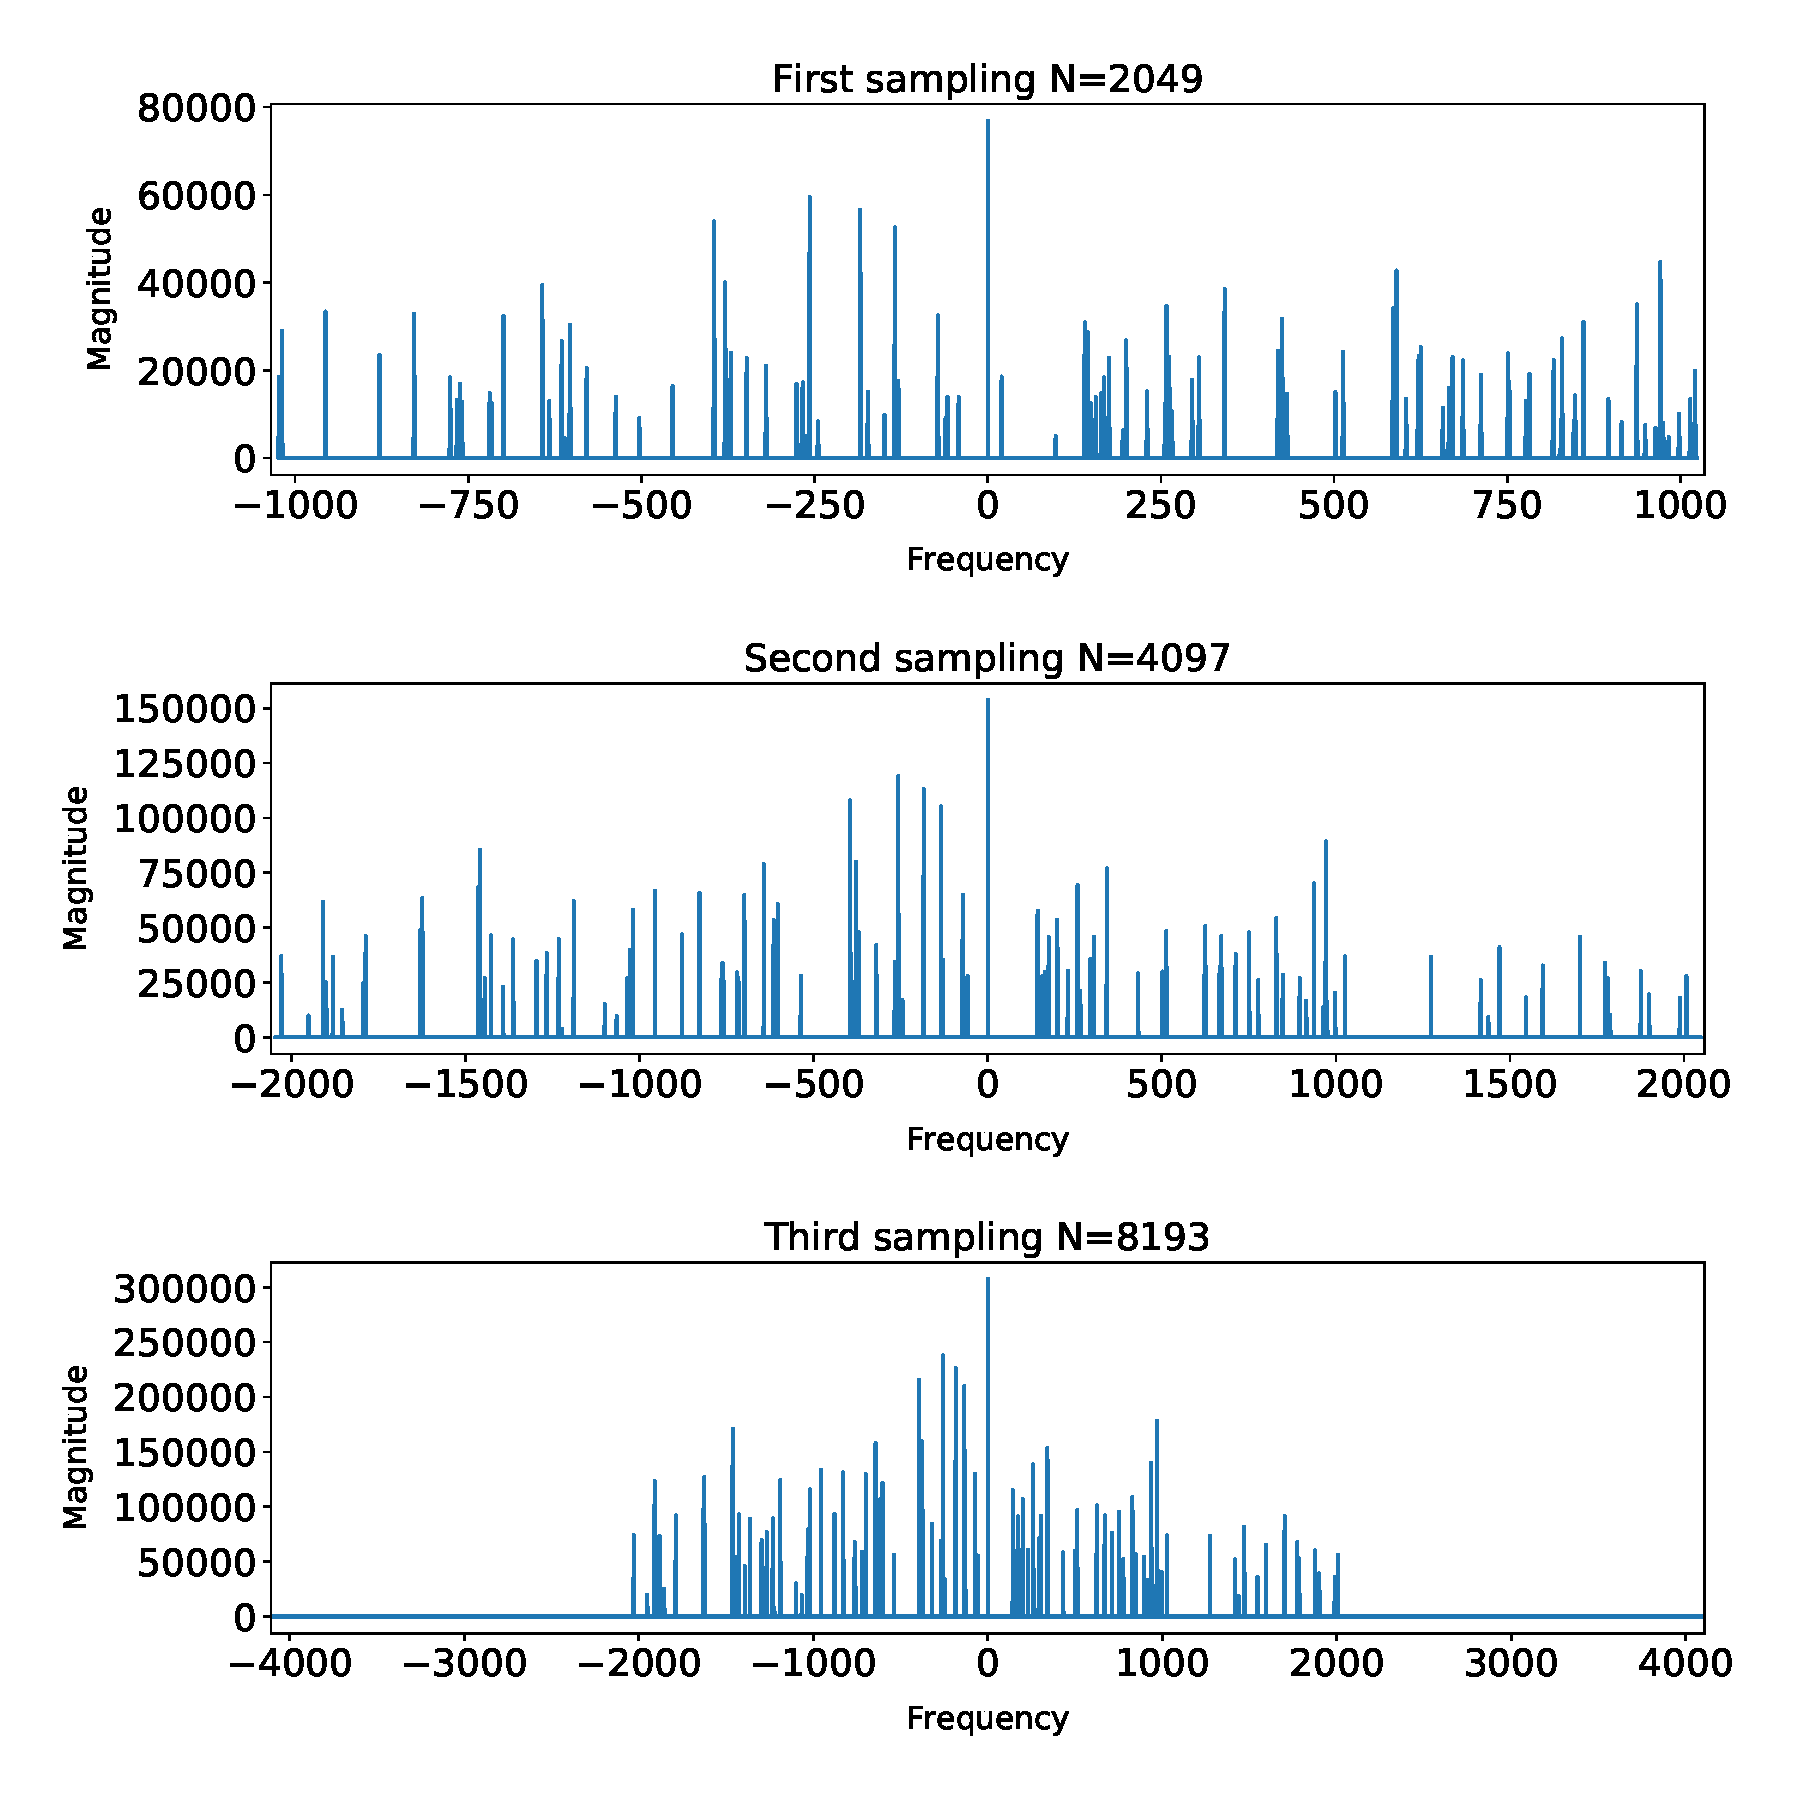
\includegraphics[width=200pt]{code/timedata/question_1.pdf}
	\end{figure}
    
   If we scale the Fourier coefficients by $N$,  to get a length invariant signal magnitude, we have the same magnitude on each plot of the signal $x$ for the corresponding
   frequencies. And as we increase the sampling frequency $\frac{1}{N}$, we have more samples:
   	
	\begin{figure}[H]
		\centering
		\captionsetup{justification=centering}
		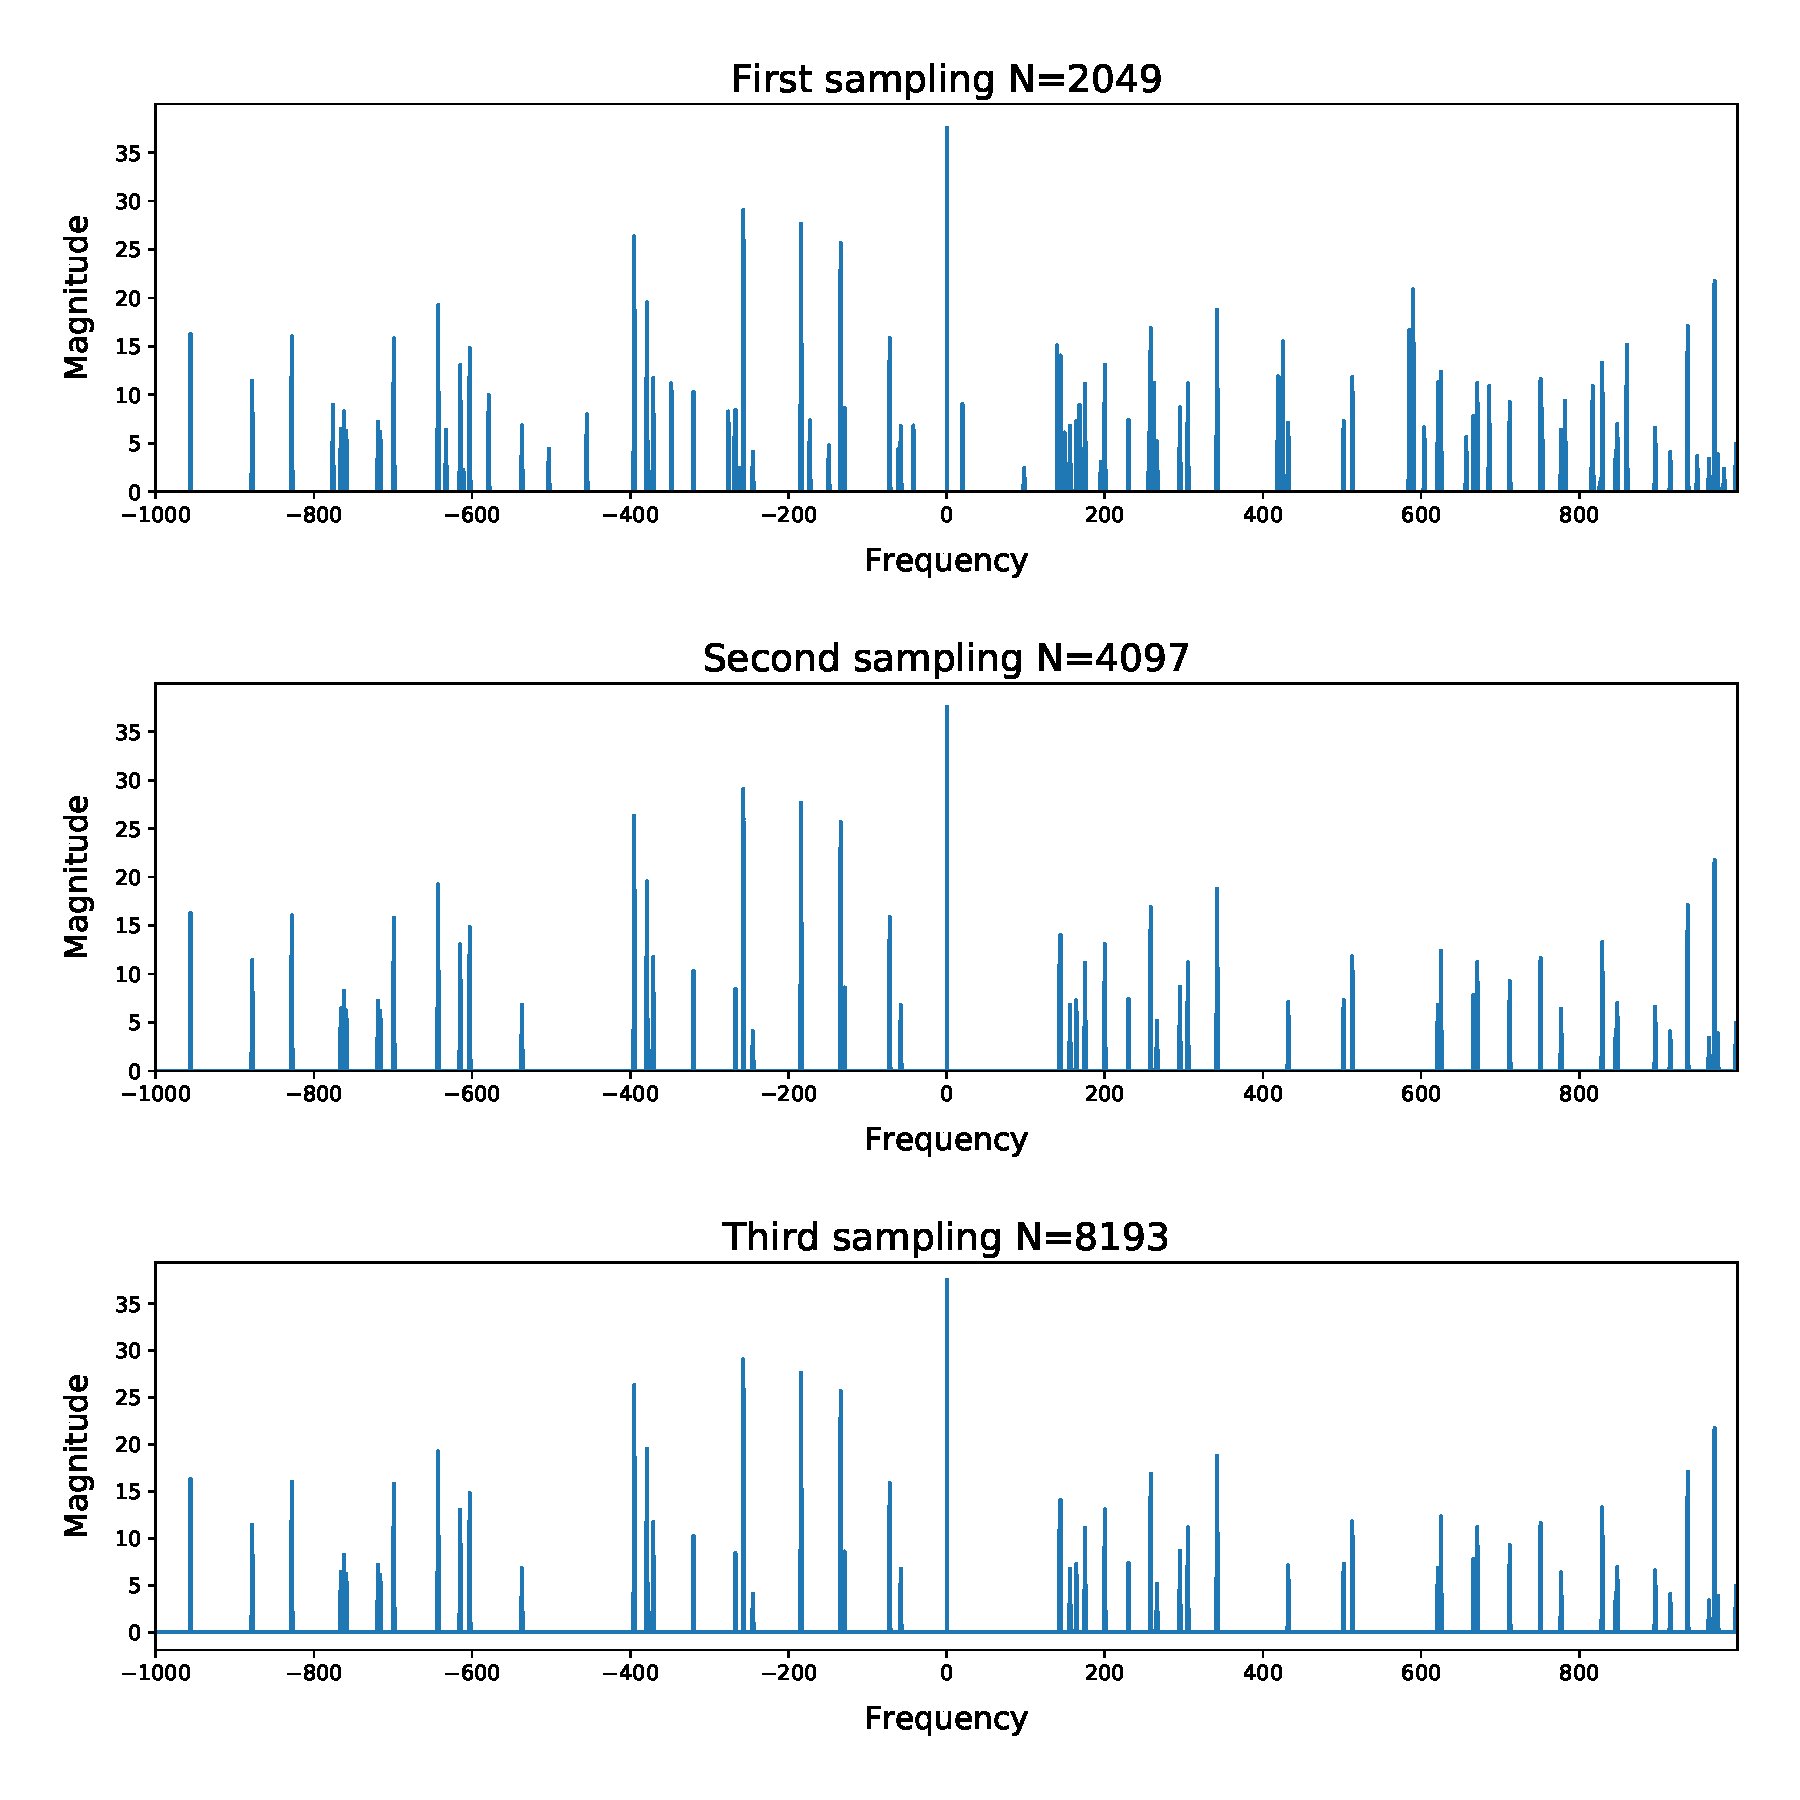
\includegraphics[width=200pt]{code/timedata/question_1_1.pdf}
	\end{figure}


  \item Assuming $k_c\leq 4096$ give the three largest $|a_k|$-values,
    along with their corresponding frequencies
    (i.e., the $k$-values). % [Hint: The largest value isn't $307237.5$.]
    
    Top $3$ largest $|a_k|$-values are:
     \begin{center}
    		\begin{tabular}{ | c | c | c | }
		\hline
			37.5 & 29.060 & 27.645 \\ 
		\hline
    	\end{tabular}
    \end{center}
    corresponding to these frequencies:
       \begin{center}
    		\begin{tabular}{ | c | c | c | }
		\hline
			0 & -257 & -184 \\ 
		\hline
    	\end{tabular}
    \end{center}

  \item Let $\hat{x}_{[2049]}$ and $\hat{x}_{[8193]}$ denote the DFT
    coefficients computed from the small and large arrays, respectively.
    Suppose you have only computed $\hat{x}_{[8193]}$
    and assume $k_c\leq4096$.
    Give a formula for $\hat{x}_{[2049]}[3]$ in terms of
    the entries of $\hat{x}_{[8193]}$ and test your formula
    on the given data.  Your formula should only require simple algebra. \\
    % [Hint: Use the aliasing formula.]
    Let $N_s=2049, N_l=8193$
    \begin{align*}
    	\hat{x}_{N}[k]	&=	\frac{1}{N} (\tilde{F}^*_{[N]} x_{[N]})[k] \\
				&=	\frac{1}{N} \sum_{j=0}^{N-1} \exp \brac{ \frac{ - i2 \pi kj}{N_s} } \sum_{m=-k_c}^{+k_c} \hat{x}[m] \exp \brac{ \frac{ - i2 \pi mj}{N_l} }\\		
				&=	\frac{1}{N} \sum_{j=0}^{N-1}  \sum_{m=-k_c}^{+k_c}  \hat{x}[m]  \exp \brac{  - i2 \pi j (\frac{k}{N_s} + \frac{m}{N_l}) } \\
				&=    \sum_{\{(N_l k + m N_s) \mod (N_s \; N_l) = 0\} } \hat{x}[m] \\
    \end{align*}
    
    
  \item True or False: Since none of the plots computed above are non-zero for
    any frequency $k$ with $|k|>2048$ it follows that
    $k_c\leq2048$. % No justification needed.
    False.High-frequency signals can fold back to a frequency within  $\leq2048$. In the question above we showed that the true signal has 
    $k_c\leq4096$ but within  $[-2048, +2048]$ aliasing can occur a different sampling rates from $N=8192$.
    
 %\item Show that for any integer $k$ with $|k|\leq k_c$, and any integer $M\geq 2k_c+1$ we must have $$\int_{0}^{1}x(t)e^{-2\pi ikt}\,dt = \frac{1}{M}\sum_{j=0}^{M-1} x(j/M)e^{-2\pi ijk/M}.$$
  \end{enumerate}

\newpage
\item (Justification of the FFT) Define the matrix
  $F_{[N]}\in\C^{N\times N}$ by
  $(F_{[N]})_{j,k}=e^{-2\pi i jk/N}$ where $0\leq j,k<N$ and $N$ is even.
  The indexing $a:b$ denotes the
  inclusive range $a,a+1,\ldots,b$, $:$ alone denotes the
  full set of indices, and $a:$ denotes all indices starting from $a$. Answer these questions to complete the proof of Lemma 4.3.
  \begin{enumerate}
  \item For any $k\geq 0$ with $2k<N$ prove a formula showing how to
    compute the rows corresponding to odd indices $(F_{[N]})_{:,2k+1}$ assuming you are given the rows for even indices $(F_{[N]})_{:,2k}$.\\ \\
    For a given element of the even row corresponding to the index $2k$: $(F_{[N]})_{j,2k}=e^{-2\pi i j 2\; k/N}, 0\leq j,k<N$ we can express the corresponding
    element $(F_{[N]})_{j,2k+1}$:
    $$
    	(F_{[N]})_{j,2k+1}=e^{-2\pi i j (2\; k + 1)/N} = e^{-2\pi i j (2\; k)/N} e^{-2\pi i j/N}  = (F_{[N]})_{j,2k} (e^{-2\pi i /N})^j
    $$
    If we define $w = e^{-2\pi i /N}$, the equality above is similar to: $w^{j (2k + 1)} = w^{j 2k} w^j$.
    
  \item For any $k\geq 0$ with $2k<N$ prove that the first half of the even columns equals the second half $(F_{[N]})_{0:N/2-1,2k}=(F_{[N]})_{N/2:,2k}$.  \\ \\
  We want to show that these vectors are the same:
  \begin{align*}
  	(F_{[N]})_{0:N/2-1,2k}	&= [1 \; w^{2k} \; w^{2 (2k)} \; \ldots \; w^{(\frac{N}{2} -1) (2k)} ]^T \\
  	(F_{[N]})_{N/2:,2k}		&= [w^{\frac{N}{2} (2k)}  \; [w^{(\frac{N}{2} + 1) (2k)}  \ldots \; w^{(N -1) (2k)} ]^T \\
  \end{align*}
  And for every element of the first half of the even column, $0 \le j \le \frac{N}{2}-1$
  \begin{align*}
  	w^N		&=	 e^{-2\pi \frac{i}{N} N} = e^{-2\pi i} = 1 \text{ ~ thus }\\ 	
  	w^{j 2k} 	&=	w^{j 2k} (w^N)^{2k} = w^{ (j +  \frac{N}{2} +  \frac{N}{2}) 2k} \\
			&= 	w^{ (j +  \frac{N}{2}) 2k} w^{(\frac{N}{2}) 2k} = w^{ (j +  \frac{N}{2}) 2k} (w^N)^k\\
			&= 	 w^{ (j +  \frac{N}{2}) 2k}
  \end{align*}
    
  \item Prove  that  the  first  half  of  the  even  columns  is  equal to  the $N/2$ DFT matrix $(F_{[N]})_{0:N/2-1,2k} = (F_{[N/2]})_{:,k}$.\\ \\
  Let $w_N = e^{\frac{-2\pi i} {N}}$ and $w_{\frac{N}{2}} =  e^{\frac{-2\pi i} {\frac{N}{2}}}$ 
  \begin{align*}
  	(F_{[N]})_{0:N/2-1,2k}	&= [1 \; w_N^{2k} \; w_N^{2 (2k)} \; \ldots \;  w_{N}^{j2k} \; \ldots \; w_N^{(\frac{N}{2} -1) (2k)} ]^T \\
  	(F_{[N/2]})_{:,k}			&= [1 \; w_{\frac{N}{2}}^k \; w_{\frac{N}{2}}^{2\;k} \; \ldots  \; w_{\frac{N}{2}}^{jk} \ldots \; w_{\frac{N}{2}}^{(N-1)k} ]^T \\
  \end{align*}
  
  For $0 \le j \le \frac{N}{2}-1$ and $0 \le k \le (N-1)$
  $$ w_{N_{j, 2k}} =  e^{\frac{-2\pi i \; j (2k)} {N}} =  e^{\frac{-2\pi i \; j k} {\frac{N}{2}}} =  w_{\frac{N}{2}_{j,k}}$$
  
   \end{enumerate}
 
 \newpage
 \item (Properties of the DFT)
  Let $F_{[N]}\in\C^{N\times N}$ denote the DFT matrix.
  \begin{enumerate}
  \item Prove that $\frac{1}{N}F_{[N]}^*$, the inverse DFT, can be
    written as $\frac{1}{N}PF_{[N]}$ for some permutation matrix $P$
    with $P^{-1}=P$.  This shows that the DFT and the inverse DFT can be
    calculated in a very similar way.
    
    The DFT matrix $F_{[N]}$, adopting the notation $w = e^{-2\pi i /N}$, is:
    $$
    \MAT{
    1 & 1 & 1 & 1 & \ldots & 1 \\
    1 & w & w^2 & w^3 & \ldots & w^{N-1} \\
    1 & w^2 & w^4 & w^6 & \ldots & w^{2 (N-1)} \\
    \vdots & \vdots & \vdots & \vdots & \ddots & \vdots \\
    1 & w^{N-1}	& w^{2(N-1)} & w^{3 (N-1)} & \ldots & w^{(N-1) (N-1)}	\\
    }
    $$
   Let $N=2l$,  $w$ is the $N^{\text{th}}$ unitary root with $w^l = -1$ and  $w^0 = w^N = 1$. All the coefficients of $F_{[N]}$ are on the unit circle equally spaced by an angle $\frac{2\pi}{N}$.
   So the conjugate of $w$ is $w^{N-1}$, $w^2$ is $w^{2 (N-2)} = w^{2N-2} = w^{N + N-2} = w^{N-2}$, up to $w^{N-1}$ which has for conjugate $w^{(N-1)(N-1)} = w^{N^2-2N+1} = w$, 
   thus taking the conjugate of the second row  gives the last row of the matrix $F_{[N]}$, 
   taking the conjugate of the third row of $F_{[N]}$ gives the $N-1$ row, 
   we keep permutating the rows following this pattern until reaching the row $N$, as a side note the row at position $l+1$ is permutated without changes.
   The permutation matrix $P$ is:
       $$
    \MAT{
    1 & 0 & 0 & 0 & \ldots & 0 \\
    0 & 0 & 0 & 0 & \ldots & 1 \\
    0 & 0 & 0 & \ldots & 1 & 0 \\
    0 & 0 & \ldots & 1 & 0 & 0 \\
    \vdots & \vdots & \vdots & \vdots & \vdots & \vdots\\
    0 & 1	& 0 & 0 & \ldots & 0	\\
    }
    $$
    If we multiply $P$ by itself, we see that  there is one-to-one relationship between the row index and the column index which happens on the diagonal,
    meaning row $i$ of $P$ multiplied with column $i$ of $P$ is $1$, however row $i$  multiplied with column $j$, where $i \neq j$ yields $0$, thus $P \; P = I$ or $P^{-1} = P$.
    In final $\frac{1}{N}F_{[N]}^* = \frac{1}{N}PF_{[N]}$
   
    
  \item Using the fact that
    $$(ABC)[j,k] = A[j,:](B)C[:,k]$$
    for any $A,B,C\in\C^{N\times N}$ and $0\leq j,k<N$ prove that
    the 2D DFT coefficients are given by
    $$(F_{[N]}XF_{[N]})[j,k] = \hat{X}[j,k],$$
    for $X\in\C^{N\times N}$.  Here we take
    $$\hat{X}[j,k] := \langle X,\psi_j\psi_k^T\rangle$$
    as the definition of $\hat{X}[j,k]$
    where $\psi_j,\psi_k\in\C^N$ are discrete
    sinusoidal basis vectors.
    [Hint: Use the trace operator.]\\
    
    From the notes on Fourier: $\psi_{j, k_1} = \exp \brac{ \frac{ i2 \pi j k_1}{N} }$  and  $\psi_{k, k_2} = \exp \brac{ \frac{ i2 \pi k k_2}{N} }$
    \begin{align*}
    	\hat{X}[j,k] 	&=	 \langle X,\psi_j\psi_k^T\rangle \\
				&=	\tr{ (\psi_j\psi_k^T)^*  X}\\
				&=	\tr{\overline{\psi_k} \psi_j^* X} \\
				&= 	\tr{\psi_j^* X \overline{\psi_k}} \\
				&= 	F_{[N]_{j,:}} X F_{[N]_{:,k}} \\ 
				&= 	(F_{[N]}XF_{[N]})[j,k] \text{ using the fact} (ABC)[j,k] = A[j,:](B)C[:,k] \\
    \end{align*}
    
  \item If $x:L_2[0,1)^2\to\C$ is real-valued, prove that the Fourier
    coefficients satisfy $\hat{x}[j,k]=\overline{\hat{x}[-j,-k]}$.\\
   % [Note: By sampling, the same property must hold for the 2D DFT.]\\
\begin{align*}
   	\hat{x}[j,k]	   	&= \PROD{x}{\phi_{j,k}^{\text{2D}}} = \int_0^1 \int_0^1 x(t_1, t_2) \exp \brac{- i2 \pi j t_1 }  \exp \brac{- 2 \pi k t_2 } \diff{t_1} \diff{t_2} \text{ ~ where we assume } T = 1\\ 	
				&=   \int_0^1 \int_0^1 x(t_1, t_2) \overline{\exp \brac{- i2 \pi (-j) t_1 }}  \;  \overline{\exp \brac{- 2 \pi (-k) t_2 }} \diff{t_1} \diff{t_2} \; x \text{being real-valued}\\
				&= \overline{\hat{x}[-j,-k]} \\
\end{align*}
   
  \end{enumerate}
  
  \newpage
  \item (Undersampling in MRI) MRI measurements can be modeled as the Fourier coefficients of tissue density (being very simplistic). An important goal is to reduce the number of Fourier coefficients, because this accelerates data acquisition, decreasing costs and improving the experience for the patient. Here we will see one of the possible pitfalls of undersampling in the Fourier domain, which is equivalent to aliasing.
 \begin{enumerate}
 \item Imagine that you only measure half of the DFT coefficients of an $N$-dimensional vector $x$.  Specifically you measure a vector $y \in \C^{N/2}$ (assume $N$ is even) that contains the Fourier coefficients corresponding to even indices. Explain how to reconstruct the vector $x_{\op{est}}$ with the smallest $\ell_2$ norm that is consistent with these measurements. Use a single multiplication with the inverse DFT matrix $\frac{1}{N}F_{[N]}^{\ast}$.\\ \\
 If we had measured all the  Fourier coefficients then $x_{\op{est}} = \frac{1}{N}F_{[N]}^{\ast} \hat{x}$, and $F_{[N]}^{\ast}$ is unitary, it preserves the norm. When  we have only $y$ which contains only the even Fourier coefficients there is an infinite number of signals solution of the previous system (it is undertermined). In order to minimize  $\ell_2$ norm of the reconstruct the vector $x_{\op{est}}$ which is proportional to the norm of the of the corresponding vector in the frequency domain, we set the odd Fourier coefficients to $0$: $x_{\op{est}} = \frac{1}{N}F_{[N]}^{\ast} [0 \; \hat{x}_2 \;0 \; \hat{x}_4 \cdots \hat{x}_N]^T$
 
 \item The script  \texttt{mr\_undersampling.py} loads the data and plots the MR image and it's Fourier coefficients. Apply your proposed reconstruction method to 2D data by completing the script \texttt{mr\_undersampling.py}.  Reconstruct the image using (1) only the even-indexed rows, (2) only the even-indexed columns, (3) only indices in even rows and columns. Report images generated using the plotting script for your under sampled Fourier coefficients and reconstructed image.  

\begin{figure}[H] 
\centering
   \begin{subfigure}[]{.5\textwidth}
   \centering
        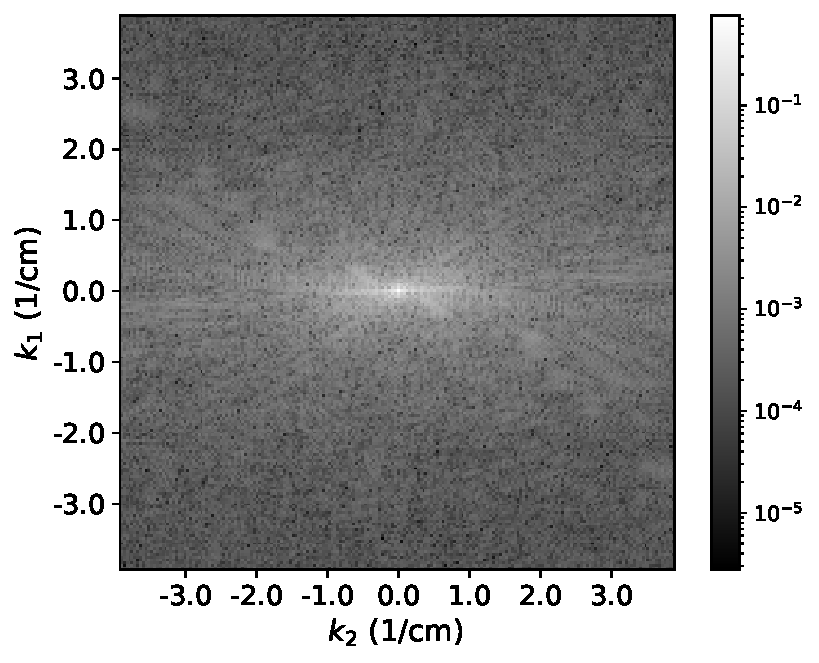
\includegraphics[width=60mm]{code/mr_undersampling/mri_samp_full_fft.pdf}
	\caption{Full sampling - frequency domain}
    \end{subfigure}%
   \begin{subfigure}[]{.5\textwidth}
   \centering   
        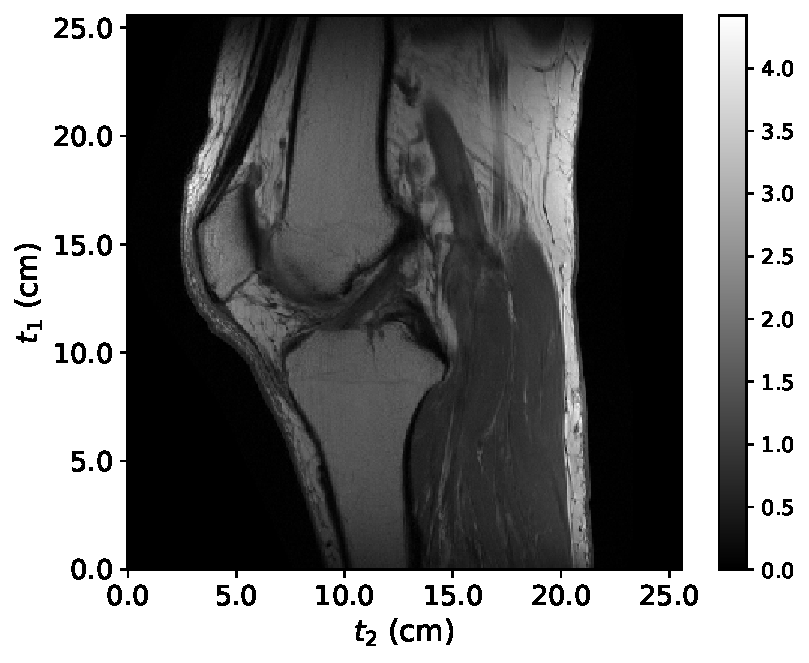
\includegraphics[width=60mm]{code/mr_undersampling/mri_samp_full.pdf}
        \caption{Full sampling - image domain}
    \end{subfigure}% 
    \hspace{4pt}%
   \begin{subfigure}[]{.5\textwidth}
   \centering
        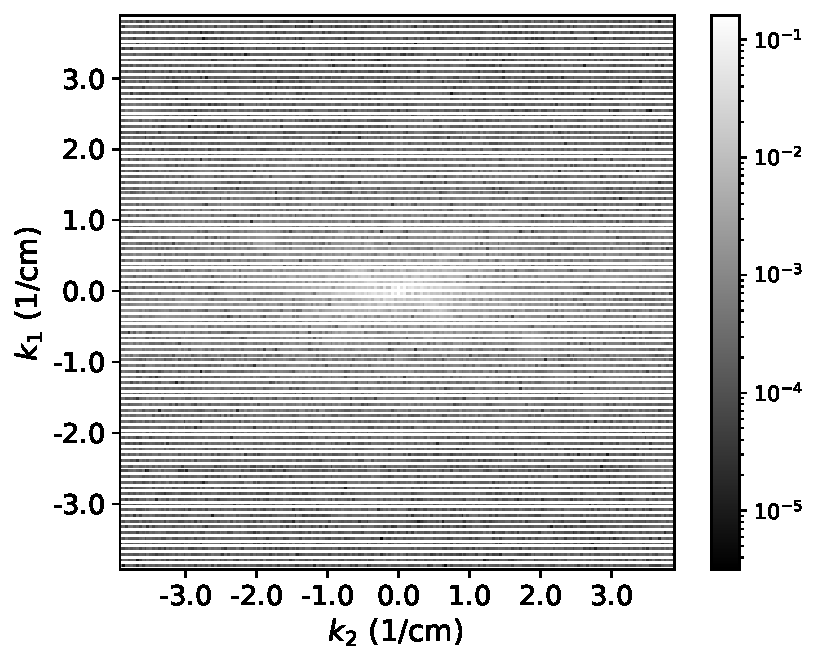
\includegraphics[width=60mm]{code/mr_undersampling/mri_undersampling_even_rows_fft.pdf}
	\caption{Even row under sampling - frequency domain}
    \end{subfigure}%
   \begin{subfigure}[]{.5\textwidth}
   \centering   
        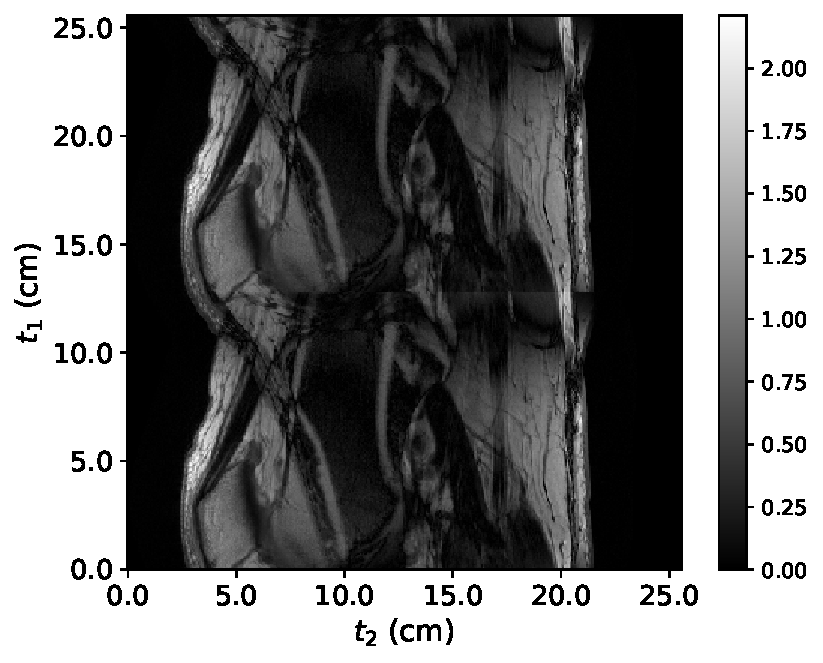
\includegraphics[width=60mm]{code/mr_undersampling/mri_even_rows_recons.pdf}
        \caption{Even row under sampling - image domain}
    \end{subfigure} 
    \hspace{4pt}%
   \begin{subfigure}[]{.5\textwidth}
   \centering
        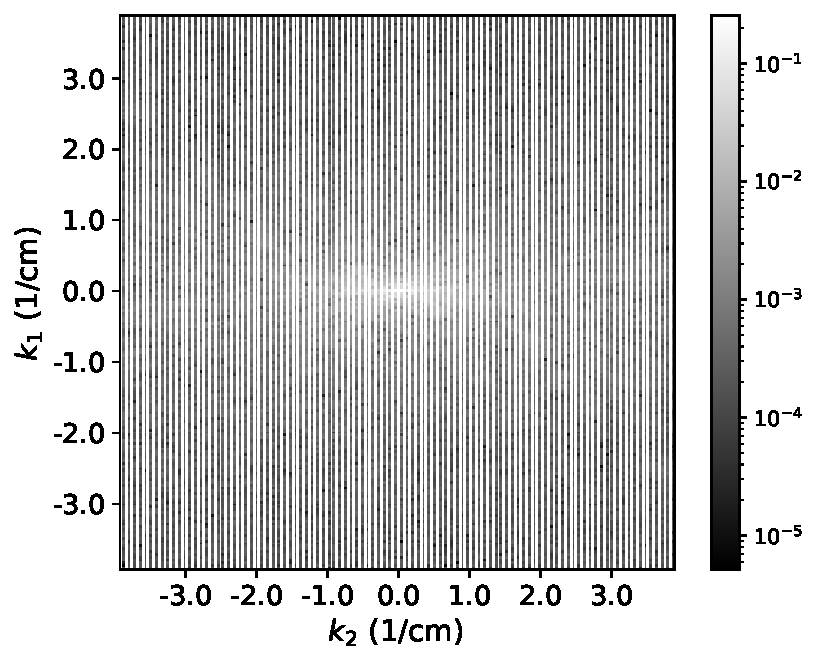
\includegraphics[width=60mm]{code/mr_undersampling/mri_undersampling_even_columns_fft.pdf}
	\caption{Even column under sampling - frequency domain}
    \end{subfigure}%
   \begin{subfigure}[]{.5\textwidth}
   \centering   
        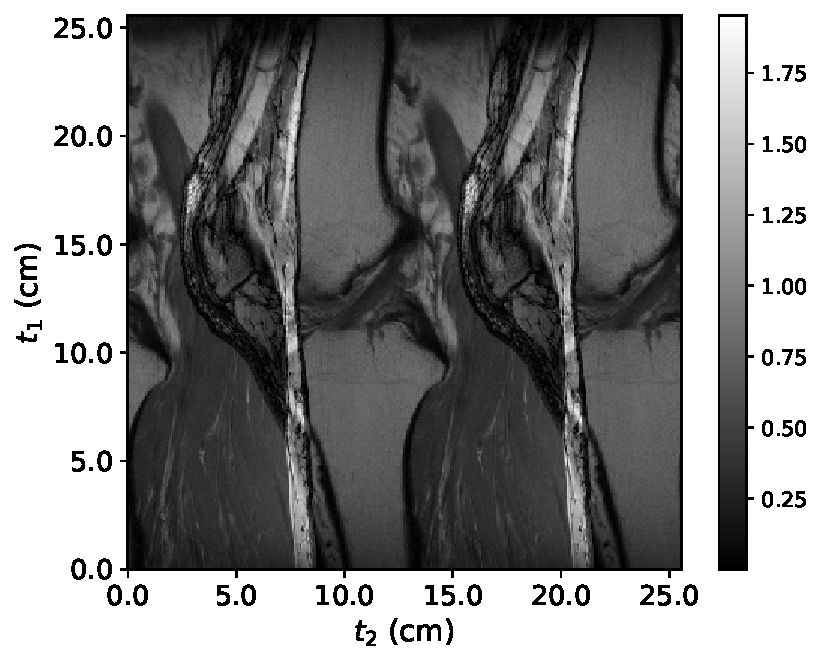
\includegraphics[width=60mm]{code/mr_undersampling/mri_even_columns_recons.pdf}
        \caption{Even column under sampling - image domain}
        \label{fig:b}    
    \end{subfigure} 
   \begin{subfigure}[]{.5\textwidth}
   \centering
        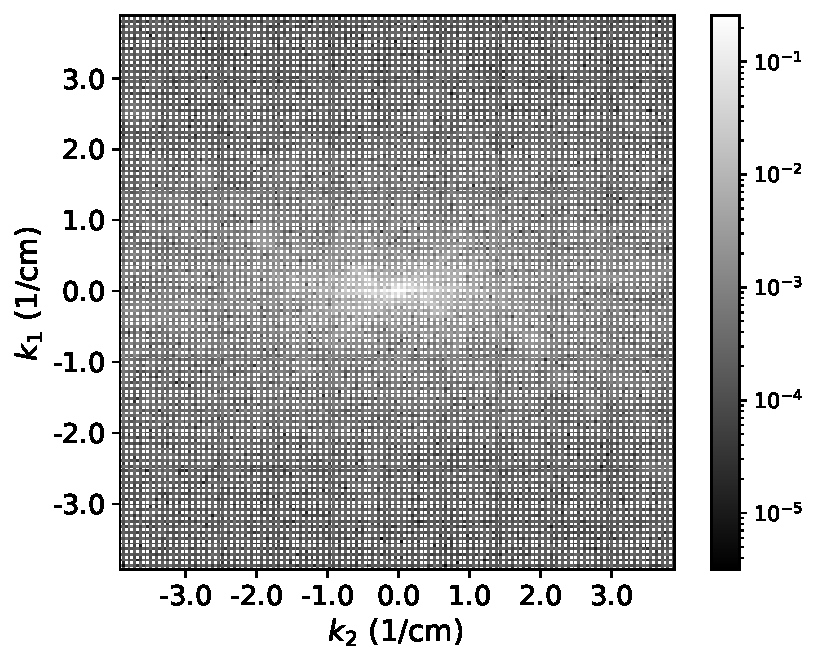
\includegraphics[width=60mm]{code/mr_undersampling/mri_undersampling_even_rows_columns_fft.pdf}
	\caption{row and column under sampling - frequency domain}
    \end{subfigure}%
   \begin{subfigure}[]{.5\textwidth}
   \centering   
        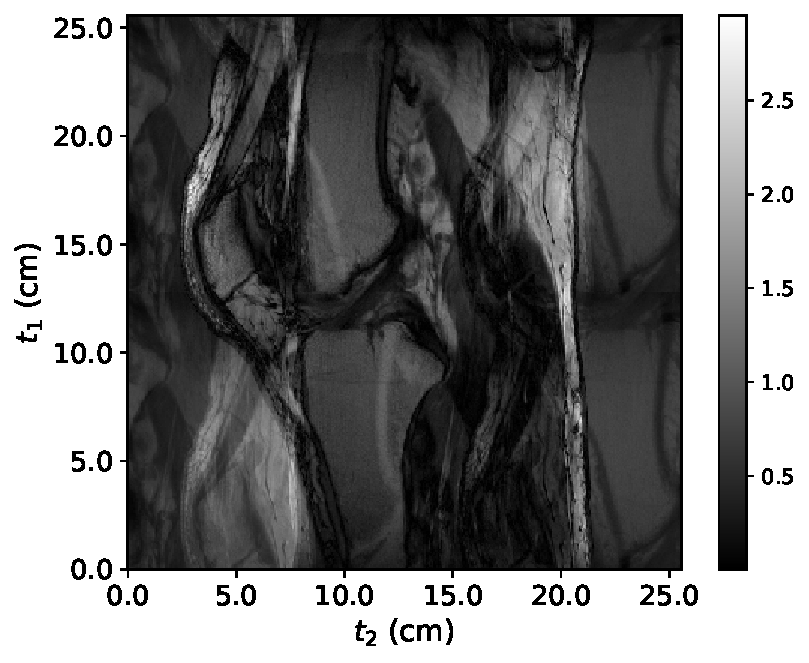
\includegraphics[width=60mm]{code/mr_undersampling/mri_even_rows_columns_recons.pdf}
        \caption{row and column under sampling - image domain}
    \end{subfigure} 
\end{figure}



  \item To explain what you are seeing, express $x_{\op{est}}$ in terms of the entries of $x$ in the 1D case. (Hint:   You might want to use some results from Problem 2(b) and 2(c).)\\ \\
  We have an aliasing, parts of the image are scrambled, if we under sample rows, up and down of the initial image are overlapping in the recovered  image, if we under sample columns
  left and right halves of the image are scrambled, the aliasing is less severe when under sampling a mixed of rows and columns. We have a duplication of the initial image and a shift. 
  From problem 2(b) and 2(c) if we sample only the even columns of $F_{[N]}$ then 
  $$
  (F_{[N]})_{\text{even columns}} =
  \MAT{
  F_{[\frac{N}{2}]} \\
   F_{[\frac{N}{2}]} }$$
 In the 1D case, measuring half of the DFT coefficients is equivalent to 
 \begin{align*}
& (F_{[N]})_{\text{even columns}} x \\
&  \MAT{
  F_{[\frac{N}{2}]} \\
   F_{[\frac{N}{2}]} } x \\
  & \MAT{
  F_{[\frac{N}{2}]} \\
   F_{[\frac{N}{2}]} } 
   \MAT{ x_{[\frac{N}{2}]} \\  x_{[\frac{N}{2}]}} \\
  & \MAT{
  F_{[\frac{N}{2}]} \\
   F_{[\frac{N}{2}]} } 
   \MAT{ x_{\text{up}} \\  x_{\text{down}}} \\
  &  F_{[\frac{N}{2}]}  [x_{\text{up}} + x_{\text{down}} \; x_{\text{up}} + x_{\text{down}}]\\
 \end{align*}
 Similarly setting all the odd entries of $\hat{x} = y$ to $0$ is equivalent to:
 \begin{align*}
 x_{\op{est}} 	&=  \frac{1}{N}F_{[\frac{N}{2}]}^{\ast} y \\
 			&=  \frac{1}{N}F_{[\frac{N}{2}]}^{\ast}   F_{[\frac{N}{2}]}   [x_{\text{up}} + x_{\text{down}} \; x_{\text{up}} + x_{\text{down}}] \\
			&=   [x_{\text{up}} + x_{\text{down}} \; x_{\text{up}} + x_{\text{down}}]
  \end{align*}
The original vector is scrambled. We can infer the same happens with an image in 2D, parts of the image are replicated and scrambled.

  \end{enumerate}

 \end{enumerate}
\end{document}
